\section{Chapter 24: The Difference-in-Differences Saga}
\subsection{Panel data and two-way fixed effects}
\sourcepages{Chapter24-25.pdf, pp. 2 and 1; p. 1 continues the assumptions at the bottom of p. 2.}
\textbf{Panel data:} repeatedly observing the same unit over time. The example compares units across time and across regions. The drawing has an early-treated group (June 1), a later-treated group (July 15), and a control group; a faint extra trajectory is labelled \emph{TWFE prediction / counterfactual}.
\begin{center}
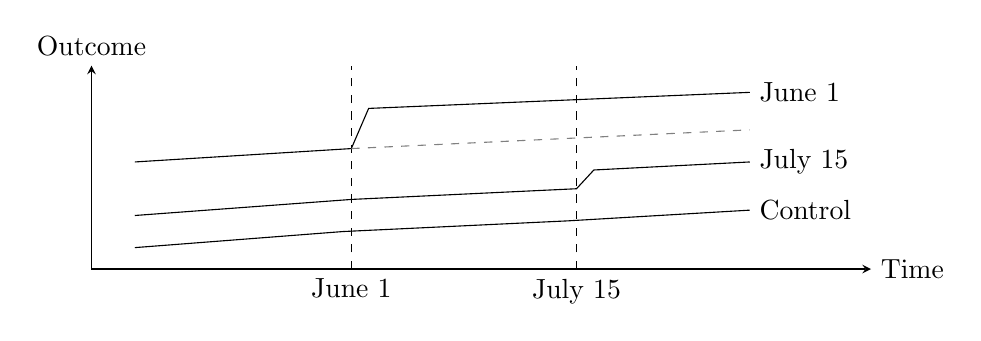
\begin{tikzpicture}[x=1.1cm,y=0.68cm,>=stealth]
\draw[->] (0,0)--(9,0) node[right]{Time};
\draw[->] (0,0)--(0,3.8) node[above]{Outcome};
\draw[dashed] (3,0)--(3,3.8);
\draw[dashed] (5.6,0)--(5.6,3.8);
\node[below] at (3,0){June 1}; \node[below] at (5.6,0){July 15};
\draw (0.5,.4)--(2.9,.7)--(5.5,.9)--(7.6,1.1) node[right]{Control};
\draw (0.5,1)--(3,1.3)--(5.6,1.5)--(5.8,1.85)--(7.6,2) node[right]{July 15};
\draw (0.5,2)--(3,2.25)--(3.2,3)--(7.6,3.3) node[right]{June 1};
\draw[gray,dashed] (3,2.25)--(7.6,2.6);
\end{tikzpicture}

{\small Schematic reconstruction of the handwritten trajectories; no numerical data are implied.}
\end{center}
Group units by their intervention date \(g\) (three groups in the example).
\notearrow{black}{Intervention start date}{Cohort label \(g\)} The target written in the notes is
\[
\operatorname{ATT}=E[Y_1\mid t>g]-E[Y_0\mid t>g].
\]
\begin{reviewnote}{qualification}{B2-003}{Define the cohort-time estimand}{Chapter24-25.pdf, pp. 2}
A precise version is \(\operatorname{ATT}(g,t)=E[Y_t(g)-Y_t(\infty)\mid G=g]\) for a treated cohort \(g\) and a post-adoption time \(t\). State whether treatment starts at \(t=g\) or only after it. An overall ATT requires aggregation weights.
\par\smallskip{\small\textit{References:} \href{https://matheusfacure.github.io/python-causality-handbook/24-The-Diff-in-Diff-Saga.html}{Primary source 1}.}
\end{reviewnote}

The model is
\[
\mathrm{Install}_{it}=\tau D_{it}+\gamma_i+\theta_t+e_{it}.
\]
Here \(i\) denotes a unit, \(t\) time, and \(e_{it}\) noise; \(\gamma_i\) is associated with \(i\) and \(\theta_t\) with \(t\). \inkblue{Estimating this by OLS gives the \textbf{two-way fixed effects (TWFE)} model.}

\paragraph{Author's annotations.}
\inkblue{At the same time, control for all characteristics.}
\notearrow{red}{Two groups and two periods}{TWFE becomes DiD.}\begin{reviewnote}{original}{B2-002}{What fixed effects actually control}{Chapter24-25.pdf, pp. 2}
Unit fixed effects absorb time-invariant differences between units; time fixed effects absorb shocks common to units at a given time. They do not control arbitrary unit-specific, time-varying confounders. Additivity and the identification assumptions still matter.
\par\smallskip{\small\textit{References:} \href{https://matheusfacure.github.io/python-causality-handbook/24-The-Diff-in-Diff-Saga.html}{Primary source 1}.}
\end{reviewnote}

\notearrow{black}{TWFE outcome model}{Residualize outcome and treatment against the same fixed effects.}
The notes write the residualized regression as
\[
\widetilde{\mathrm{Install}}_{it}=\tau\widetilde D_{it}+e_{it},
\]
with the following demeaning expressions:
\begin{align*}
\widetilde{\mathrm{Install}}_{it}
 &=\mathrm{Install}_{it}
 -\underbrace{\frac1T\sum_{t=0}^{T}\mathrm{Install}_{it}}_{\textcolor{red}{\text{time average}}}
 -\underbrace{\frac1N\sum_{i=0}^{N}\mathrm{Install}_{it}}_{\textcolor{red}{\text{unit average}}},\\
\widetilde D_{it}
 &=D_{it}-\frac1T\sum_{t=0}^{T}D_{it}-\frac1N\sum_{i=0}^{N}D_{it}.
\end{align*}
\begin{reviewnote}{original}{B2-004}{Double demeaning needs the grand mean}{Chapter24-25.pdf, pp. 2, 6}
For a balanced panel indexed by \(i=1,\ldots,N\), \(t=1,\ldots,T\), use
\[
\widetilde z_{it}=z_{it}-\bar z_{i\cdot}-\bar z_{\cdot t}+\bar z_{\cdot\cdot},\qquad z\in\{Y,D\}.
\]
Here \(\bar z_{i\cdot}=T^{-1}\sum_{s=1}^Tz_{is}\), \(\bar z_{\cdot t}=N^{-1}\sum_{j=1}^Nz_{jt}\), and \(\bar z_{\cdot\cdot}=(NT)^{-1}\sum_{j,s}z_{js}\). The added grand mean makes each row and column mean zero. Omitting it shifts each transformed variable by a constant; if the final regression includes an intercept, the slope is unchanged. It is nevertheless not the exact fixed-effect residual, and a no-intercept regression need not give the same slope. With unbalanced panels, use the actual fixed-effect projection rather than this simple formula.
\par\smallskip{\small\textit{References:} \href{https://matheusfacure.github.io/python-causality-handbook/24-The-Diff-in-Diff-Saga.html}{Primary source 1}, \href{https://matheusfacure.github.io/python-causality-handbook/25-Synthetic-Diff-in-Diff.html}{Primary source 2}.}
\end{reviewnote}


\subsection{Death: Failures over Effect Heterogeneity}
TWFE often has bias when effects are heterogeneous. The fixed-effects model without time effects is written as
\[
y_{it}=\tau D_{it}+\gamma_i+e_{it}.
\]
The assumptions listed in the notebook are:
\begin{enumerate}
\item \textbf{Functional form:} no heterogeneous effect over time (constant effects); linearity in the covariates; additive fixed effects.
\item \textbf{Strict exogeneity:} parallel trends; no anticipation; no unobserved time-varying confounders; past treatment does not affect the current outcome (no carryover); past outcomes do not affect current treatment (no feedback).
\end{enumerate}
The second item is the left-page continuation connected by the arrow at the foot of the main page.
\notearrow{black}{Strict-exogeneity list at the foot of p. 2}{Continuation on p. 1: anticipation, confounding, carryover, and feedback.}\begin{reviewnote}{qualification}{B2-005}{Strict exogeneity and DiD assumptions}{Chapter24-25.pdf, pp. 1, 2}
In a static fixed-effect regression, a standard condition is \(E[e_{it}\mid D_{i1},\ldots,D_{iT},\gamma_i]=0\) (with the other regressors also conditioned on). Parallel trends and no anticipation are potential-outcome restrictions used for DiD; they are not interchangeable with the whole list. Dynamic effects can be allowed by changing the model and estimand.
\par\smallskip{\small\textit{References:} \href{https://matheusfacure.github.io/python-causality-handbook/24-The-Diff-in-Diff-Saga.html}{Primary source 1}.}
\end{reviewnote}


\sourcepages{Chapter24-25.pdf, p. 3.}
Continuing the previous point: suppose the treatment effect is heterogeneous over time, and the treatment response is gradual (from \(0.1,0.2,\ldots\), increasing from day to day). The ATT estimated by TWFE is then biased.
The drawing labels the early-treated group \(1\), the late-treated group \(2\), and the never-treated group \(3\). Decomposing TWFE into several \(2\times2\) DiDs gives:
\[
1-3:\ \checkmark,\quad
2-3:\ \checkmark,\quad
1-2:\ \checkmark,\quad
2-1:\ \text{??}
\]
The second member of each comparison is the control. \textbf{Author's intuition:} if the early-treated group \(1\) is used as the control, the model thinks that the untreated outcome \(Y_0\) would have risen in parallel with that group's earlier trajectory. \notearrow{blue}{Estimated untreated trajectory}{The blue curve is \(\widehat Y_0\) for the late-treated group.}
\begin{center}
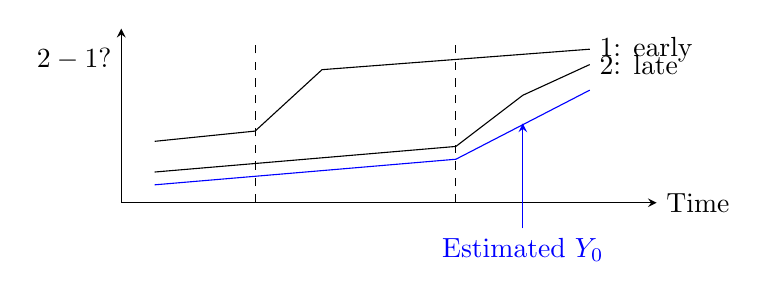
\begin{tikzpicture}[x=.85cm,y=.65cm,>=stealth]
\draw[->] (0,0)--(8,0) node[right]{Time}; \draw[->] (0,0)--(0,3.4);
\draw[dashed] (2,0)--(2,3.2); \draw[dashed] (5,0)--(5,3.2);
\draw (0.5,1.2)--(2,1.4)--(3,2.6)--(7,3) node[right]{1: early};
\draw (0.5,.6)--(5,1.1)--(6,2.1)--(7,2.7) node[right]{2: late};
\draw[blue] (.5,.35)--(5,.85)--(7,2.2);
\node[blue,below] (b) at (6,-.5){Estimated \(Y_0\)};
\draw[->,blue] (b.north)--(6,1.55);
\node[left] at (0,2.8){\(2-1\)?};
\end{tikzpicture}
\end{center}
This schematic restores the comparison-to-curve relationship; line heights are illustrative.

The notebook attributes this shorthand to Goodman-Bacon (2019):
\[
\operatorname*{plim}_{n\to\infty}\widehat\tau^{\mathrm{TWFE}}
 =\mathrm{VWATT}-\Delta\mathrm{ATT}.
\]
\notearrow{blue}{Bias: the extent to which ATT changes over time}{\(\Delta\mathrm{ATT}\)}
\inkblue{If the effect increases over time, as in the drawing, the bias is downward; in the opposite case it is upward. \textbf{Author's warning:} with negative effects that become more negative over time, even the estimated sign can be wrong.}\begin{reviewnote}{qualification}{B2-006}{The direction-of-bias claim refers to the illustrated comparison}{Chapter24-25.pdf, pp. 3}
The sketch explains contamination when already-treated units serve as controls. The sign and magnitude of the aggregate TWFE discrepancy depend on cohort effects, their dynamics, and the regression weights; the illustration is not a universal sign theorem.
\par\smallskip{\small\textit{References:} \href{https://matheusfacure.github.io/python-causality-handbook/24-The-Diff-in-Diff-Saga.html}{Primary source 1}.}
\end{reviewnote}


\subsection{Event-study design}
Rewrite TWFE using event-time indicators. The notebook writes the following lead/lag expansion (coefficient and index labels retained):
\begin{align*}
Y_{it}={}&\tau^{-K}D_{ik}^{<-K}
 +\sum_{k=-K}^{-2}\tau^{\mathrm{lead}}D_{it}^{k}
 +\sum_{k=0}^{L}\gamma_k^{\mathrm{lag}}D_{it}^{k}\\
 &+\gamma_k^{L+}D_{it}^{>L}+\gamma_i+e_{it},\\
D_{it}^{k}={}&\mathbf1\{t-\mathrm{Cohort}_i=k\}.
\end{align*}
\notearrow{black}{\(D_{it}^{k}=\mathbf1\{t-\mathrm{Cohort}_i=k\}\)}{One in relative period \(k\), zero otherwise.}
\notearrow{blue}{Add a variable measuring distance from treatment start}{The event-time indicator \(D_{it}^{k}\).}
This is labelled a \emph{partial improvement}.\begin{reviewnote}{original}{B2-007}{A complete lead/lag regression}{Chapter24-25.pdf, pp. 3}
A conventional specification, omitting the reference period \(k=-1\), is
\begin{align*}
Y_{it}={}&\alpha_i+\theta_t+\beta_{<-K}\mathbf1\{t-G_i<-K\}\\
&+\sum_{k=-K}^{-2}\beta_k\mathbf1\{t-G_i=k\}
+\sum_{k=0}^{L}\beta_k\mathbf1\{t-G_i=k\}\\
&+\beta_{>L}\mathbf1\{t-G_i>L\}+e_{it}.
\end{align*}
Never-treated units have all event-time indicators zero. The faint source separator before the unit effect is rendered as a plus; the inconsistent subscripts are a source-notation problem.
\par\smallskip{\small\textit{References:} \href{https://matheusfacure.github.io/python-causality-handbook/24-The-Diff-in-Diff-Saga.html}{Primary source 1}.}
\end{reviewnote}
\begin{reviewnote}{qualification}{B2-008}{Event-time dummies alone do not solve heterogeneous effects}{Chapter24-25.pdf, pp. 3}
With staggered adoption and heterogeneous effects, a lead or lag coefficient can combine effects from other relative periods, and apparent pretrends can arise from effect heterogeneity. Use an estimator with explicit valid cohort comparisons when interpreting these coefficients causally.
\par\smallskip{\small\textit{References:} \href{https://arxiv.org/abs/1804.05785}{Primary source 1}.}
\end{reviewnote}


\subsection{Enlightenment: A Flexible Functional Form}
\sourcepages{Chapter24-25.pdf, p. 4.}
A new model gives every individual a treatment effect at every time:
\[
\mathrm{Installs}_{it}
 =\sum_{i=0}^{N}\sum_{t=0}^{T}\tau_{it}D_{it}+\gamma_i+\theta_t+e_{it}.
\]
There are too many parameters. Instead, assign an effect to each group \(g\) at each time:
\[
\mathrm{Installs}_{it}
 =\sum_{g=0}^{G}\sum_{t=0}^{T}\tau_{gt}D_{it}+\gamma_i+\theta_t+e_{it}.
\]
This is marked as a better version. Reduce the parameters further by removing pre-treatment coefficients and the control-group coefficients:
\[
\mathrm{Installs}_{it}
 =\sum_{g=q}^{G}\sum_{t\geq g}^{T}\tau_{gt}D_{it}+\gamma_i+\theta_t+e_{it}.
\]
Cohorts with \(g<q\) are defined as controls.
\notearrow{blue}{Manually create cohort dummies: \((0,1),(1,0),\ldots\)}{The cohort-by-time treatment terms.}\begin{reviewnote}{original}{B2-009}{Write cohort-by-time indicators explicitly}{Chapter24-25.pdf, pp. 4}
For observation \((i,s)\), the intended expansion is
\[
Y_{is}=\alpha_i+\theta_s+
\sum_{g\in\mathcal G}\sum_{t\geq g}\tau_{g,t}
\mathbf1\{G_i=g\}\mathbf1\{s=t\}+e_{is}.
\]
The cohort and calendar-time indicators are essential. This repairs the displayed notation, not the identification assumptions.
\par\smallskip{\small\textit{References:} \href{https://matheusfacure.github.io/python-causality-handbook/24-The-Diff-in-Diff-Saga.html}{Primary source 1}.}
\end{reviewnote}
\begin{reviewnote}{qualification}{B2-010}{Control cohorts must supply untreated comparisons}{Chapter24-25.pdf, pp. 4}
If \(g\) is an actual adoption date, an earlier cohort may already be treated and cannot automatically serve as an untreated control. Use never-treated units, or not-yet-treated units during the relevant comparison window, with the appropriate parallel-trends and no-anticipation assumptions. The handbook example labels cohorts that adopt after the observed window as controls.
\par\smallskip{\small\textit{References:} \href{https://matheusfacure.github.io/python-causality-handbook/24-The-Diff-in-Diff-Saga.html}{Primary source 1}.}
\end{reviewnote}

Remaining limitations:
\begin{enumerate}
\item Treatment effects can change as time passes; this was not considered before.
\item DiD and TWFE must satisfy the parallel-trends assumption. The restriction is very strong.
\end{enumerate}
\notearrow{black}{DiD and TWFE}{Require the relevant parallel-trends restriction.}

\section{Chapter 25: Synthetic Difference-in-Differences}
\subsection{Representing panel data}
\sourcepages{Chapter24-25.pdf, p. 5.}
There are multiple units over multiple periods, with treated and untreated observations mixed together. In \(D\), \textbf{rows are times and columns are units}:
\[
D=\begin{pmatrix}
0&0&0&\cdots&0&0\\
0&0&0&\cdots&0&0\\
\vdots&\vdots&\vdots&&\vdots&\vdots\\
0&0&0&\cdots&1&1\\
0&0&0&\cdots&1&1
\end{pmatrix}.
\]
The final columns identify the treated units.
\notearrow{black}{Columns containing ones after adoption}{Treated units} The note calls this \emph{one-time treatment} and stars the design requirement: once a unit is treated, it does not return to an untreated state.
\begin{reviewnote}{qualification}{B2-011}{The four-block matrix needs a common treatment block}{Chapter24-25.pdf, pp. 5}
The displayed four-block representation assumes a common pre/post split for the included treated units. Under staggered adoption, construct valid cohort or period subpanels first, as in the later notes.
\par\smallskip{\small\textit{References:} \href{https://arxiv.org/pdf/1812.09970}{Primary source 1}, \href{https://matheusfacure.github.io/python-causality-handbook/25-Synthetic-Diff-in-Diff.html}{Primary source 2}.}
\end{reviewnote}


\paragraph{Representation 1: synthetic control.}
Collapse the display into four blocks:
\[
D=\begin{pmatrix}0&0\\0&1\end{pmatrix},\qquad
Y=\begin{pmatrix}
Y_{\mathrm{pre,co}}&Y_{\mathrm{pre,tr}}\\
Y_{\mathrm{post,co}}&Y_{\mathrm{post,tr}}
\end{pmatrix}.
\]
Here pre means before treatment, post after treatment, co control group, and tr treatment group.
\paragraph{Representation 2: DiD.}
Use a long table with columns for unit, time, outcome, whether the unit belongs to the treatment group, and whether it has already been treated.
The observed outcomes are
\[
Y=\begin{pmatrix}
Y(0)_{\mathrm{pre,co}}&Y(0)_{\mathrm{pre,tr}}\\
Y(0)_{\mathrm{post,co}}&Y(1)_{\mathrm{post,tr}}
\end{pmatrix},
\]
and
\[
\operatorname{ATT}=Y(1)_{\mathrm{post,tr}}
-\underbrace{Y(0)_{\mathrm{post,tr}}}_{\text{missing}}.
\]

\subsection{Revisiting DiD and synthetic controls}
\sourcepages{Chapter24-25.pdf, pp. 6 and 7; p. 7 supplies the two comparison sketches.}
The DiD regression is
\[
Y_{it}=\beta_0+\beta_1\mathrm{Post}_t+\beta_2\mathrm{Treated}_i
+\beta_3\mathrm{Treated}_i\mathrm{Post}_t+e_{it}.
\]
Its assumption is
\[
E[Y(0)_{\mathrm{post,co}}-Y(0)_{\mathrm{pre,co}}]
=E[Y(0)_{\mathrm{post,tr}}-Y(0)_{\mathrm{pre,tr}}].
\]
That is, in the absence of treatment the control and treatment groups have the same trend.

Rewrite the estimator in a form comparable to SDID:
\[
\widehat\tau^{\mathrm{did}}
=\operatorname*{argmin}_{\mu,\alpha,\beta,\tau}
\left\{\sum_{i=1}^{N}\sum_{t=1}^{T}
[Y_{it}-(\mu+\alpha_i+\beta_t+\tau D_{it})]^2\right\}.
\]
The notes connect this to demeaning:
\begin{align*}
\widetilde Y_{it}
&=Y_{it}-\overline Y_i-\overline Y_t
=Y_{it}-T^{-1}\sum_{t=0}^{T}Y_{it}-N^{-1}\sum_{i=0}^{N}Y_{it},\\
\widetilde D_{it}
&=D_{it}-\overline D_i-\overline D_t
=D_{it}-T^{-1}\sum_{t=0}^{T}D_{it}-N^{-1}\sum_{i=0}^{N}D_{it}.
\end{align*}
This looks like synthetic controls, but lacks the weights.
\notearrow{black}{Demeaning \(Y\) and \(D\)}{The fixed-effects least-squares criterion.}
\begin{reviewnote}{original}{B2-004}{Repeated double-demeaning omission}{Chapter24-25.pdf, p. 6}
Add the grand mean and use consistent summation endpoints, as corrected in B2-004 above.
\par\smallskip{\small\textit{References:} \href{https://matheusfacure.github.io/python-causality-handbook/24-The-Diff-in-Diff-Saga.html}{Primary source 1}, \href{https://matheusfacure.github.io/python-causality-handbook/25-Synthetic-Diff-in-Diff.html}{Primary source 2}.}
\end{reviewnote}

For synthetic control, estimate weights using pre-treatment outcomes:
\[
\widehat w^{\mathrm{sc}}
=\operatorname*{argmin}_{w}
\|\overline y_{\textcolor{blue}{\mathrm{pre,tr}}}-Y_{\mathrm{pre,co}}w_{\mathrm{co}}\|_2^2,
\qquad \sum_iw_i=1,\quad w_i>0\quad\forall i.
\]
\begin{reviewnote}{original}{B2-012}{Allow zero donor weights}{Chapter24-25.pdf, pp. 6, 8, 10}
The standard simplex constraint is \(w_i\geq0\), \(\sum_{i\in\mathrm{co}}w_i=1\), and similarly \(\lambda_t\geq0\), \(\sum_{t\in\mathrm{pre}}\lambda_t=1\). Zero weights are allowed. The open simplex \(w_i>0\) can exclude the optimizer. On pp. 8 and 10 the handwritten constraints additionally omit the summation sign: individual weights are not all equal to one. The formulas below restore the intended sum-to-one constraint.
\par\smallskip{\small\textit{References:} \href{https://matheusfacure.github.io/python-causality-handbook/25-Synthetic-Diff-in-Diff.html}{Primary source 1}, \href{https://arxiv.org/pdf/1812.09970}{Primary source 2}.}
\end{reviewnote}

Here \(Y_{\mathrm{pre,co}}\) is a \(T_{\mathrm{pre}}\times N_{\mathrm{co}}\) outcome matrix: columns are units and rows are time periods. The vector \(w_{\mathrm{co}}\) has size \(N_{\mathrm{co}}\times1\). Each entry of \(\overline y_{\mathrm{pre,tr}}\) is the average of the treated units at a pre-treatment time.

\paragraph{Author's annotations.}
\inkblue{Fit a synthetic control to the treated group; this is similar to linear regression.} After treatment, use the control outcomes and the fitted weights:
\[
y_{\mathrm{sc}}=Y_{\mathrm{co}}\widehat w^{\mathrm{sc}}.
\]
This gives a good estimate of \(Y(0)_{\mathrm{post,tr}}\). Thus
\[
\widehat\tau=\overline y_{\mathrm{post,tr}}-\overline y_{\mathrm{post,sc}}.
\]
Rewrite it as
\[
\widehat\tau^{\mathrm{sc}}
=\operatorname*{argmin}_{\beta,\tau}
\left\{\sum_{i=1}^{N}\sum_{t=1}^{T}
(Y_{it}-\beta_t-\tau D_{it})^2\widehat w_i^{\mathrm{sc}}\right\}.
\]
The pre-treatment fitting step provides control-group weights; each treated unit has weight \(1/N_{\mathrm{tr}}\). \notearrow{blue}{No overall intercept \(\mu\); no unit effects \(\alpha_i\)}{The SC weighted regression criterion above.}

\paragraph{Left-page visual intuition (p. 7).}
The DiD sketch shifts a trajectory into a parallel comparison; the handwritten comment says this amplifies the effect in the illustrated case. In the SC sketch, pre-treatment data generate weights and hence a synthetic untreated treatment group. Use the same weights to compute post-treatment outcomes, and estimate the effect from the difference between the two post-treatment values. The curves closely track before treatment, then separate.
\notearrow{black}{Pre-treatment fit}{Weights \(\widehat w\)}
\notearrow{black}{Control outcomes and the same weights after treatment}{Synthetic post-treatment outcome, then its gap from the treated outcome.}
\begin{center}
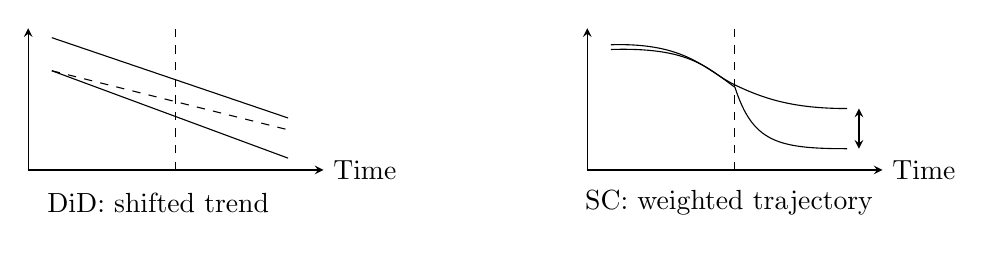
\begin{tikzpicture}[x=0.75cm,y=0.6cm,>=stealth]
\draw[->] (0,0)--(5,0) node[right]{Time};
\draw[->] (0,0)--(0,3);
\draw[dashed] (2.5,0)--(2.5,3);
\draw (0.4,2.8)--(4.4,1.1);
\draw (0.4,2.1)--(4.4,0.25);
\draw[dashed] (0.4,2.1)--(4.4,0.85);
\node at (2.2,-0.7){DiD: shifted trend};
\begin{scope}[xshift=7.1cm]
\draw[->] (0,0)--(5,0) node[right]{Time};
\draw[->] (0,0)--(0,3);
\draw[dashed] (2.5,0)--(2.5,3);
\draw (0.4,2.65) .. controls (1.7,2.7) and (2,2.1) .. (2.5,1.8)
.. controls (3,1.5) and (3.5,1.3) .. (4.4,1.3);
\draw (0.4,2.55) .. controls (1.7,2.6) and (2,2.2) .. (2.5,1.75)
.. controls (2.8,0.6) and (3.2,.45) .. (4.4,.45);
\draw[<->] (4.6,.45)--(4.6,1.3);
\node at (2.4,-0.7){SC: weighted trajectory};
\end{scope}
\end{tikzpicture}

{\small Schematic reconstructions of the author's sketches.}
\end{center}


\subsection{Combining the two: synthetic DiD}
\sourcepages{Chapter24-25.pdf, pp. 8 and 10 (upper and middle portions).}
\inkred{\(\star\)} The starred heading combines the synthetic-control weighted criterion and the DiD fixed-effects criterion:
\[
\widehat\tau^{\mathrm{sdid}}
=\operatorname*{argmin}_{\mu,\alpha,\beta,\tau}
\left\{\sum_{i=1}^{N}\sum_{t=1}^{T}
[Y_{it}-(\mu+\alpha_i+\beta_t+\tau D_{it})]^2
\underbrace{\widehat w_i^{\mathrm{sdid}}}_{\textcolor{red}{\text{unit weight}}}
\underbrace{\widehat\lambda_t^{\mathrm{sdid}}}_{\textcolor{red}{\text{time weight}}}\right\}.
\]
\paragraph{Time weights.}
Fit the average post-treatment outcome of the controls from their pre-treatment outcomes:
\[
\widehat\lambda^{\mathrm{sdid}}
=\operatorname*{argmin}_{\lambda}
\|\overline y_{\textcolor{blue}{\mathrm{post,co}}}
-(\lambda_{\mathrm{pre}}Y_{\mathrm{pre,co}}+\lambda_0)\|_2^2,
\qquad \sum_t\lambda_t=1,\quad\lambda_t>0.
\]
\begin{itemize}
\item \(Y_{\mathrm{pre,co}}\) is \(T_{\mathrm{pre}}\times N_{\mathrm{co}}\); rows are times and columns are units.
\item \(\overline y_{\mathrm{post,co}}\) is a \(1\times N_{\mathrm{co}}\) row vector. Each entry is a control unit's time-averaged outcome after treatment.
\item \(\lambda_{\mathrm{pre}}\) is a \(1\times T_{\mathrm{pre}}\) row vector, with a weight for every pre-treatment period. \(\lambda\) is a time weight.
\end{itemize}
The active replacement sketch at the bottom of p. 8 multiplies along the time dimension: prepend a row of ones to the matrix for the intercept, and fit \(\overline y_{\mathrm{post,co}}\) from the weighted pre-treatment rows to obtain \(\lambda_t\).
\begin{center}
\begin{tikzpicture}[>=stealth,node distance=22mm]
\node (x) {\(\begin{pmatrix}\mathbf1^{\mathsf T}\\Y_{\mathrm{pre,co}}\end{pmatrix}\)};
\node[right=of x] (fit) {\((\lambda_0,\lambda_{\mathrm{pre}})\)};
\node[right=of fit,blue] (y) {\(\overline y_{\mathrm{post,co}}\)};
\draw[->] (x)--node[above,font=\small]{time fit}(fit);
\draw[->] (fit)--(y);
\end{tikzpicture}
\end{center}

\paragraph{Unit weights.}
The small diagram at the top of p. 10 connects control/pre to control/post by \(\lambda\), and control/pre to treated/pre by \(w\), giving the corresponding treated/post comparison.
\begin{center}
\begin{tikzpicture}[>=stealth,node distance=14mm and 28mm,blue]
\node (a) {Control/pre}; \node[right=of a] (b) {Control/post};
\node[below=of a] (c) {Treated/pre}; \node[below=of b] (d) {Treated/post};
\draw[->] (a)--node[above]{\(\lambda\)}(b); \draw[->] (a)--node[left]{\(w\)}(c);
\draw[->] (b)--(d); \draw[->] (c)--(d);
\end{tikzpicture}
\end{center}
\begin{align*}
\widehat w^{\mathrm{sdid}}
=\operatorname*{argmin}_{w}\ \big\{
&\|\overline y_{\textcolor{blue}{\mathrm{pre,tr}}}
-(Y_{\mathrm{pre,co}}w_{\mathrm{co}}+w_0)\|_2^2\\
&+\zeta^2T_{\mathrm{pre}}\|w_{\mathrm{co}}\|_2^2\big\},
\qquad \sum_iw_i=1,\quad w_i>0,\\
\zeta&=(N_{\mathrm{tr}}T_{\mathrm{post}})^{1/4}
\widehat\sigma(\Delta_{it}),\\
\Delta_{it}&=Y_{it}-Y_{i,t-1}.
\end{align*}
Here \(\Delta_{it}\) is the first difference and \(\widehat\sigma(\Delta_{it})\) its standard deviation.

\paragraph{Author's annotations.}
\notearrow{red}{The \(L_2\) penalty spreads the nonzero weights more widely}{\(\zeta^2T_{\mathrm{pre}}\|w_{\mathrm{co}}\|_2^2\)}
\notearrow{blue}{Compared with SC: (1) an intercept; (2) an \(L_2\) penalty}{The SDID unit-weight fit.} \notearrow{blue}{There is an intercept}{\(w_0\)}
The implementation instruction says to add a row of ones \emph{before \(\overline y_{\mathrm{pre,tr}}\)} as an intercept and perform the regression.
\begin{reviewnote}{original}{B2-013}{Put the intercept in the design matrix}{Chapter24-25.pdf, pp. 10}
For the unit-weight fit, \(\overline y_{\mathrm{pre,tr}}\) is a \(T_{\mathrm{pre}}\)-vector and the design is
\[
X=[\,\mathbf1_{T_{\mathrm{pre}}}\ \ Y_{\mathrm{pre,co}}\,].
\]
Add a \emph{column} of ones to the predictors, not a row to the outcome. Fit \((w_0,w_{\mathrm{co}})\); constrain and penalize only the donor weights, not the intercept. By contrast, the row-vector time-weight convention on p. 8 correctly prepends a row of ones to \(Y_{\mathrm{pre,co}}\).
\par\smallskip{\small\textit{References:} \href{https://matheusfacure.github.io/python-causality-handbook/25-Synthetic-Diff-in-Diff.html}{Primary source 1}, \href{https://arxiv.org/pdf/1812.09970}{Primary source 2}.}
\end{reviewnote}
\begin{reviewnote}{qualification}{B2-014}{Estimate the scale from untreated pre-treatment data}{Chapter24-25.pdf, pp. 10}
The standard SDID construction uses first differences of control-unit outcomes during the pre-treatment period to estimate \(\widehat\sigma\). Using treated post-intervention outcomes can let the effect influence the regularization scale. The positive fourth-root factor \((N_{\mathrm{tr}}T_{\mathrm{post}})^{1/4}\) in the notes is correct.
\par\smallskip{\small\textit{References:} \href{https://arxiv.org/pdf/1812.09970}{Primary source 1}.}
\end{reviewnote}


For the treated units and post-treatment times, use uniform weights \(1/N_{\mathrm{tr}}\) and \(1/T_{\mathrm{post}}\), respectively. \textbf{Author's intuition:} compared with SC, SDID focuses on data near the period when the intervention takes effect.\begin{reviewnote}{qualification}{B2-015}{Unclear wording in the SDID intuition}{Chapter24-25.pdf, pp. 10}
The temporal reading above is plausible, but the middle characters remain unclear. Mathematically, time weights make weighted control pre-treatment outcomes predict control post-treatment outcomes; they do not select observations by closeness to an unknown treatment effect, and they need not select only recent periods.
\par\smallskip{\small\textit{References:} \href{https://matheusfacure.github.io/python-causality-handbook/25-Synthetic-Diff-in-Diff.html}{Primary source 1}, \href{https://arxiv.org/pdf/1812.09970}{Primary source 2}.}
\end{reviewnote}


\subsection{Time-effect heterogeneity and staggered adoption}
\sourcepages{Chapter24-25.pdf, p. 10 (lower portion), then the p. 9 supplement.}
SDID makes it easy to estimate an effect for each period: simply run the procedure multiple times. In these handwritten matrices, subscripts on the zeros and ones identify the period.
\paragraph{\inkred{Time-effect heterogeneity.}}
The example is
\[
D=\begin{pmatrix}
0_1&0_1&0_1\\0_2&0_2&0_2\\0_3&0_3&1_3\\0_4&0_4&1_4
\end{pmatrix}.
\]
Applying SDID gives an average ATT over periods 3 and 4.
\notearrow{black}{The full matrix \(D\)}{SDID: average ATT over periods 3 and 4.} To estimate these periods separately, use
\[
D_1=\begin{pmatrix}0_1&0_1&0_1\\0_2&0_2&0_2\\0_3&0_3&1_3\end{pmatrix},
\qquad
D_2=\begin{pmatrix}0_1&0_1&0_1\\0_2&0_2&0_2\\0_4&0_4&1_4\end{pmatrix}.
\]

\paragraph{\inkred{Staggered adoption: left-page supplement.}}
The notebook gives
\[
D=\begin{pmatrix}
0_1&0_1&0_1\\0_2&0_2&0_2\\0_3&0_3&1_3\\0_4&1_4&1_4
\end{pmatrix}.
\]
The first decomposition is
\[
D_1=\begin{pmatrix}0_1&0_1&0_1\\0_2&0_2&0_2\\0_4&1_4&1_4\end{pmatrix},
\qquad
D_2=\begin{pmatrix}0_1&0_1&0_1\\0_2&0_2&0_2\\0_3&0_3&1_3\end{pmatrix}.
\]
Weight the ATT from \(D_1\) by \(2/3\), and the ATT from \(D_2\) by \(1/3\).
\notearrow{black}{Split the original treatment matrix by period}{Two treated cells in period 4 and one in period 3: weights \(2/3\) and \(1/3\).} Alternatively, split by treated cohort:
\[
D_1=\begin{pmatrix}0_1&0_1\\0_2&0_2\\0_3&0_3\\0_4&1_4\end{pmatrix},
\qquad
D_2=\begin{pmatrix}0_1&0_1\\0_2&0_2\\0_3&1_3\\0_4&1_4\end{pmatrix}.
\]
The example underneath says: California, treated for 12 years; others, 8 years \(\times3\). The weighting calculation is
\[
\mathrm{ATT}_0\frac{12}{36}
+\left(\sum\mathrm{ATT}\right)\frac13\frac{3\times8}{36}.
\]
This preserves the author's treatment-duration weighting illustration.
\begin{reviewnote}{qualification}{B2-017}{Treatment-cell weights define the aggregate target}{Chapter24-25.pdf, pp. 9, 10}
The \(2/3,1/3\) weights count treated cells. Likewise, \(12/36\) and \(24/36\) average the California and three-other-unit effects over their observed treated durations, with equal period and unit weights. Other target populations can require different aggregation weights. Use genuinely untreated donor observations in each subpanel.
\par\smallskip{\small\textit{References:} \href{https://matheusfacure.github.io/python-causality-handbook/25-Synthetic-Diff-in-Diff.html}{Primary source 1}, \href{https://arxiv.org/pdf/1812.09970}{Primary source 2}.}
\end{reviewnote}


\subsection{Placebo variance estimation}
\sourcepages{Chapter24-25.pdf, p. 11.}
Compared with SC, the notebook describes SDID as having lower error bars. SDID captures variation in outcomes over time and across units. This improves the SDID confidence interval and applies to a single treated unit.
\begin{reviewnote}{qualification}{B2-018}{Precision is not uniformly better}{Chapter24-25.pdf, pp. 11}
SDID can improve precision and robustness in suitable designs; smaller valid standard errors than SC are not a universal guarantee. Estimated weights also contribute uncertainty, so an ordinary weighted-regression standard error is not automatically the SDID standard error.
\par\smallskip{\small\textit{References:} \href{https://matheusfacure.github.io/python-causality-handbook/25-Synthetic-Diff-in-Diff.html}{Primary source 1}, \href{https://arxiv.org/pdf/1812.09970}{Primary source 2}.}
\end{reviewnote}


For each control unit, pretend it received treatment and use SDID to estimate a placebo ATT. The notes write
\[
\widehat V_{\tau}^{\mathrm{placebo}}
=B^{-1}\sum_{b=1}^{B}
\left(\widehat\tau^{(b)}-\overline\tau^{(b)}\right)^2,
\qquad
\tau\in\widehat\tau^{\mathrm{sdid}}
\pm z_{\alpha/2}\sqrt{\widehat V_\tau}.
\]
\notearrow{black}{Variance of placebo ATT estimates}{SDID placebo variance \(\widehat V_\tau\), then a confidence interval.} A parenthetical annotation says this is the same as SC.
\begin{reviewnote}{qualification}{B2-019}{Define the placebo mean and the interval convention}{Chapter24-25.pdf, pp. 11}
For \(B\) placebo estimates define \(\overline\tau^{\mathrm{pl}}=B^{-1}\sum_b\widehat\tau^{(b)}\) and
\[
\widehat V^{\mathrm{pl}}=B^{-1}\sum_b(\widehat\tau^{(b)}-\overline\tau^{\mathrm{pl}})^2.
\]
If \(z_p=\Phi^{-1}(p)\), the normal-approximation interval is \(\widehat\tau\pm z_{1-\alpha/2}\sqrt{\widehat V^{\mathrm{pl}}}\). The handwritten \(z_{\alpha/2}\) can instead mean a positive upper-tail critical value; its convention is unstated. A confidence interval is a random set with a coverage claim, not a certainty that the realized interval contains \(\tau\).
\par\smallskip{\small\textit{References:} \href{https://arxiv.org/pdf/1812.09970}{Primary source 1}.}
\end{reviewnote}
\begin{reviewnote}{qualification}{B2-020}{Single-treated-unit placebo inference needs assumptions}{Chapter24-25.pdf, pp. 11}
The placebo construction borrows noise information from controls. It needs comparable noise across units (the SDID paper requires cross-unit homoskedasticity for this argument), suitable donor samples, and a justified distributional approximation. It can fail when the treated unit has different noise variability. For more than one treated unit, each placebo assignment should reproduce the treated-group size.
\par\smallskip{\small\textit{References:} \href{https://arxiv.org/pdf/1812.09970}{Primary source 1}.}
\end{reviewnote}


\section{Appendix: Debiasing and Prediction}
\sourcepages{Chapter24-25.pdf, p. 12.}
A heading note links the treatment of non-randomized data to \textbf{propensity scores} and \textbf{orthogonalization}.
\subsection{Debiasing with orthogonalization}
\notearrow{blue}{Same as Chapter 22}{Orthogonalization / residualizing the variables.} All features are contained in \(X\).
\begin{enumerate}
\item Take the first group of features and fit
\[
y_i=\theta_0+\theta_1X_{1i}+e_i.
\]
Obtain the residual
\[
y_i^*=y_i-(\widehat\theta_0+\widehat\theta_1X_{1i}).
\]
\item Use the first group of features to predict the second group:
\[
X_{2i}=\gamma_0+\gamma_1X_{1i}+e_i.
\]
Obtain the residual
\[
X_{2i}^*=X_{2i}-(\widehat\gamma_0+\widehat\gamma_1X_{1i}).
\]
\item Regress the outcome residual on the feature residual:
\[
y_i^*=\beta_0+\beta_2X_{2i}^*+e_i.
\]
\end{enumerate}

\subsection{Debiasing with propensity scores}
\sourcepages{Chapter24-25.pdf, p. 13.}
\notearrow{blue}{See Chapter 11}{Propensity-score weighting.} Weight each unit. For binary treatment,
\[
w_i=\frac{T}{P(T=1\mid X)}+\frac{1-T}{1-P(T=1\mid X)}.
\]
The next formula, labelled \emph{continuous} in the manuscript, is
\[
w_i=\sum_{k=0}^{K}\frac{\mathbf1\{T=k\}}{P(T=k\mid X)}.
\]
\begin{reviewnote}{original}{B2-021}{The displayed extension is categorical}{Chapter24-25.pdf, pp. 13}
This expression is for a discrete treatment with categories \(0,\ldots,K\). For a genuinely continuous dose, \(P(T=k\mid X)=0\) at an individual point in the usual continuous model; generalized propensity methods use a conditional density and require a separately specified dose-response estimand and estimator.
\par\smallskip{\small\textit{References:} \href{https://matheusfacure.github.io/python-causality-handbook/Debiasing-with-Propensity-Score.html}{Primary source 1}.}
\end{reviewnote}


\paragraph{Author's intuition.}
\begin{inkblock}{blue}
A unit with a high probability of treatment that nevertheless remains untreated essentially resembles a treated unit but is observed in the control group. It can be used to estimate \(Y_0\mid T=1\).
\end{inkblock}\begin{reviewnote}{qualification}{B2-022}{ATE and ATT weights differ}{Chapter24-25.pdf, pp. 13}
Under consistency, conditional exchangeability, and positivity, the displayed inverse-probability weights target ATE comparisons. For an ATT comparison, treated units receive weight 1 and controls receive \(e(X)/(1-e(X))\), with suitable normalization. A high-propensity control helps represent the treated covariate distribution, but it is not literally a treated unit.
\par\smallskip{\small\textit{References:} \href{https://matheusfacure.github.io/python-causality-handbook/Debiasing-with-Propensity-Score.html}{Primary source 1}.}
\end{reviewnote}

If propensity scores are unavailable, estimate them using the probability of receiving treatment as the target, with machine learning. A small numerical illustration mentions 20\%, 0.2, and receiving an email marked \(1\); the rest of that short line is unclear in the scan.
\begin{reviewnote}{qualification}{B2-023}{Email example remains partly unreadable}{Chapter24-25.pdf, pp. 13}
The legible quantities are retained; no extra probability calculation or causal claim is inferred from the missing words.
\end{reviewnote}


\paragraph{Weaknesses of propensity scores.}
\begin{enumerate}
\item When the propensity score is very small (\(e<0.05\)), the weight is too large: the observation effectively appears too many times and strongly influences the debiased dataset. The note mentions manual trimming. \inkblue{\textbf{High variance.}}
\item \textbf{Positivity or common support:} there must be enough overlap between the characteristics of treated and control units. If overlap is too limited, propensity-score adjustment does a poor job of removing the association.
\end{enumerate}
\begin{inkblock}{red}
Manual intervention is not very advisable because it can introduce excessive subjective bias; do not extrapolate to population subsets where positivity does not hold.
\end{inkblock}\begin{reviewnote}{qualification}{B2-024}{Large weights and trimming}{Chapter24-25.pdf, pp. 13}
For binary ATE weighting, small \(e\) inflates treated-unit weights \(1/e\), while \(e\) near one inflates control weights \(1/(1-e)\). Trimming can be a principled, prespecified response to limited overlap, but changes the population being studied and must be reported. Good propensity prediction alone does not establish causal exchangeability.
\par\smallskip{\small\textit{References:} \href{https://matheusfacure.github.io/python-causality-handbook/Debiasing-with-Propensity-Score.html}{Primary source 1}.}
\end{reviewnote}


\subsection{When prediction fails}
\sourcepages{Chapter24-25.pdf, p. 14.}
Prediction and causality. This is a heading-only page; no further notes are written beneath it.
